%//==============================--@--==============================//%
\subsection{P3 | Modelo de crescimento do tumor}
\label{subsec:P3}
%//==============================--A--==============================//%
\vspace{-0.5em}
\subsubsection[a) Pontos de equilíbrio]{a) Pontos de equilíbrio (para $u = 0$)}% 'TeX não gosta de math nos títulos, nifty trick
\label{subsubsec:P3a}

No equilíbrio, $V(t)$ é constante, e consequentemente, a primeira derivada é nula.
\vskip -0.75em
$$
    \begin{cases}
        \dot{V}(t) = 0\\
        u = 0
    \end{cases}\implies
    aV\left(1 - \frac{V}{K_T} \right) = 0 \implies V = 0 \lor V = K_T = 10\ \text{mm}^3
$$
%//==============================--B--==============================//%
\subsubsection[b) Análise da monotonia da variável V (para u = 0)]{b) Análise da monotonia da variável $V$ (para $u = 0$)}% 'TeX não gosta de math nos títulos, nifty trick
\label{subsubsec:P3b}
\vspace{-1.5em}
\hspace*{-2.25em}
\begin{tabular}{c c}
    \noindent\begin{minipage}[t]{0.5\textwidth}
        \begin{figure}[H]
            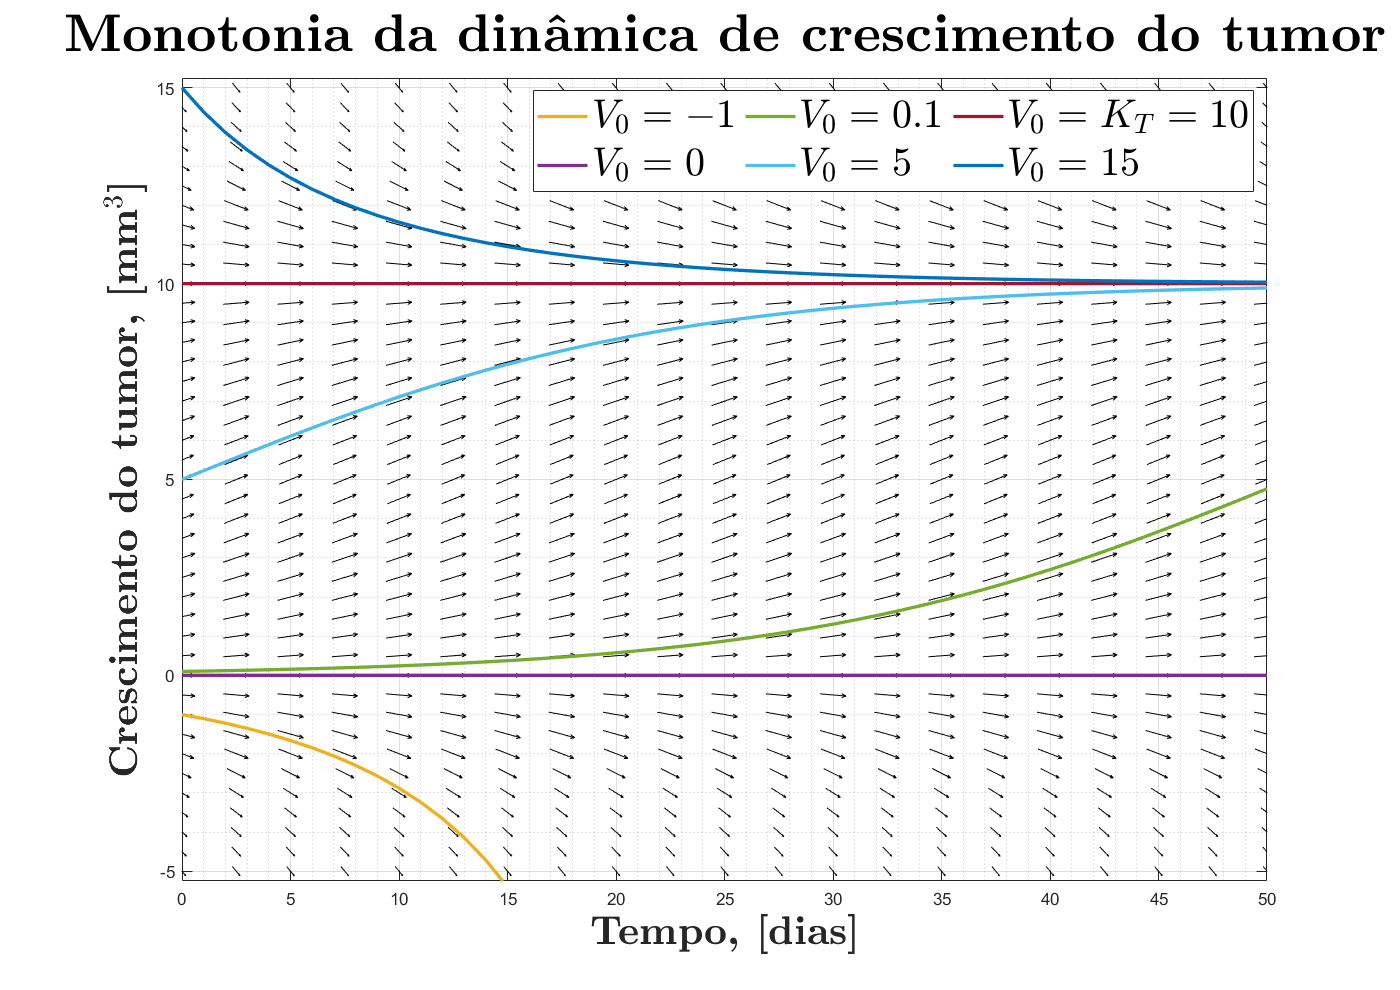
\includegraphics[width = 1\linewidth]{img/perguntas/P3/P3-monotonia.png}
            \hspace*{1.65em}\begin{minipage}{1\linewidth}
                \caption{Evolução do volume do tumor para\\ diferentes valores iniciais.}
                \label{fig:P3-monotonia}
            \end{minipage}
        \end{figure}
    \end{minipage} &\
    \hspace*{-1em}\noindent\begin{minipage}[t]{0.5\textwidth}
            \vspace{1.75em}
            \hspace*{1.35em}\begin{minipage}{1\linewidth}
                \captionof{table}{Tabela de monotonia do crescimento\\ do tumor $V(t)$ para $u = 0$.}
                \label{tab:P3-monotonia}
            \end{minipage}
            \renewcommand\arraystretch{1.5}
            \hspace*{-0.5em}\begin{tabular}{*{8}{c}}
                \toprule
                $V(t)$ & $-\infty$ & & $0$ & & $K_T$ & & $+\infty$ \\
                \midrule
                $\dot{V}(t)$ & $-$ & $-$ & 0 & $+$ & 0 & $-$ & $-$ \\
                %$\Ddot{V}(t)$ & $-$ & $-$ & 0 & $+$ & 0 & $-$ & $-$ \\
                $V(t)$ & \multicolumn{2}{c}{$\color{blue} \pmb{\searrow}$} & $eq_{min}$ & $\color{blue} \pmb{\nearrow}$ & $eq_{max}$ & \multicolumn{2}{c}{$\color{blue} \pmb{\searrow}$} \\
                \bottomrule
            \end{tabular}
            \vspace{0.3em}
            \[ \therefore \text{\textbf{Monotonia de }} V(t) \]
            \[ \raisebox{0.2 em}{$\drsh$}\ \text{\textbf{Decrescente}:}\ V \in\ \left]-\infty, 0\right[\, \cup\, \left]K_T, +\infty\right[ \]
            \vspace{-1.7em}
            \[ \hspace*{-5em} \raisebox{0.2 em}{$\drsh$}\ \text{\textbf{Crescente}:}\ V \in\ \left]0, K_T\right[ \]      
    \end{minipage}
\end{tabular}

Ao iniciar a simulação com um volume de $V_0 = 0$, não há crescimento, e o volume mantém-se em zero. Para um volume inicial de $0<V(t_0)<K_T$, verifica-se então um crescimento; no entanto, é atingido um \textit{plateau}, quando $V(t)$ se aproxima de $K_T$ (\textit{saturation level}/\textit{carrying capacity}). Para $V_0 = K_T$, também não ocorre crescimento, e o volume permanece neste valor (vide a \hyperref[subsubsec:P3a]{secção anterior}). Finalmente, se começarmos com um volume superior a $K_T$, o volume decresce até eventualmente se encontrar na vizinhança da solução de equilíbrio assintóticamente estável.

Note-se que foi incluída uma secção de $V$'s negativos (apesar de não ter qualquer significado num contexto real), de modo a explicitar o comportamento "perto" de $V_0 = 0$ (solução de equilíbrio assintóticamente instável).

%//==============================--C--==============================//%
\subsubsection[c) Poderá V assumir valores negativos mediante valores de u?]{c) Poderá $V$ assumir valores negativos mediante valores de $u \in [0; 1]$?}% 'TeX não gosta de math nos títulos, nifty trick 
\label{subsubsec:P3c}
Seja $0 \leq u(t) \leq u_{max}$ e $V(t_0) > 0$. Tendo em conta a equação logística:
\vspace{-0.25em}
\begin{equation}
    \dot{V}(t) = aV\left(1-\frac{V}{K_T}\right) - buV = \left[ a\left( 1-\frac{V}{K_T} \right) - bu \right]V = [a-bu]V-\left[\frac{a}{K_T}\right]V^2
\end{equation}

\vspace{-0.25em}
\noindent verifica-se que os \underline{pontos de equilíbrio} passam a ser:
\vspace{-0.75em}
$$
    V = 0\quad\lor\quad V = \chi \delequal K_T-\frac{buK_T}{a}
$$
\vspace{-2.25em}
%\iffalse
\begin{figure}[!h]
    \centering
    \begin{subfigure}[b]{0.25\textwidth}
    \centering
    \resizebox{1\textwidth}{!}{%
        \begin{tikzpicture}
            \begin{axis}[
                axis lines = center,
                xlabel = {$V(t)$},
                ylabel = {$\dot{V}(t)$},
                y label style={at = {(0.13,1.00575)}},
                grid style=dashed,
                grid=none,
                ticks=none
            ]

            \addplot[
                domain=(-3):(7), 
                samples=300, 
                color=darkgray,
                dashed
            ]
            {-x*(x-4)};

            % pontos
            \node[label={55:{\color{darkgray} $\pmb{\chi}$}},inner sep=2pt] at (3.4,-3) {};
            \node[label={55:{\color{darkgray} $\pmb{0}$}},inner sep=2pt] at (0,-3) {};

            % signs
            \node[label={0:{\color{red} $\pmb{-}$}},inner sep=2pt] at (5.2,-5.8) {};
            \node[label={0:{\color{red} $\pmb{-}$}},inner sep=2pt] at (-2.2,-5.8) {};
            \node[label={0:{\color{red} $\pmb{+}$}},inner sep=2pt] at (1.5,1.65) {};

            % arrows
            \draw[->] (axis cs:3.3, 3.7) -- (axis cs:4.2, 0.7);
            \draw[->] (axis cs:5.1, -3.7) -- (axis cs:4.55, -0.7);
            
            %\addlegendentry{}
            \end{axis}
        \end{tikzpicture}
    }%
    \caption{Caso com $u \in [0, 0.09[$}
    \end{subfigure}\qquad
    \begin{subfigure}[b]{0.25\textwidth}
    \centering
    \resizebox{1\textwidth}{!}{%
        \begin{tikzpicture}
            \begin{axis}[
                axis lines = center,
                xlabel = {$V(t)$},
                ylabel = {$\dot{V}(t)$},
                y label style={at = {(0.35,1.005)}},
                grid style=dashed,
                grid=none,
                ticks=none,
                ymax=1.9,
                ymin=-10
            ]

            \addplot[
                domain=(-15):(15), 
                samples=300, 
                color=darkgray,
                dashed
            ]
            {-x^2};

            % pontos
            \node[label={55:{\color{darkgray} $\pmb{0 \equiv \chi}$}},inner sep=2pt] at (0,-0.25) {};

            % signs
            \node[label={0:{\color{red} $\pmb{-}$}},inner sep=2pt] at (1.7,-2.3) {};
            \node[label={0:{\color{red} $\pmb{-}$}},inner sep=2pt] at (-2.4,-2.3) {};

            % arrows
            \draw[->] (axis cs:1.5, -1.7) -- (axis cs:1, -0.5);

            %\addlegendentry{}
            \end{axis}
        \end{tikzpicture}
    }%
    \caption{Caso com $u = a = 0.09$}
    \end{subfigure}\qquad
    \begin{subfigure}[b]{0.25\textwidth}
    \centering
    \resizebox{1\textwidth}{!}{%
        \begin{tikzpicture}
            \begin{axis}[
                axis lines = center,
                xlabel = {$V(t)$},
                x label style={at = {(1,0.7)}},
                ylabel = {$\dot{V}(t)$},
                grid style=dashed,
                grid=none,
                ticks=none
            ]

            \addplot[
                domain=(-7):(3), 
                samples=300, 
                color=darkgray,
                dashed
            ]
            {-x*(x+4)};

            % pontos
            \node[label={55:{\color{darkgray} $\pmb{\chi}$}},inner sep=2pt] at (-4.3,-3) {};
            \node[label={55:{\color{darkgray} $\pmb{0}$}},inner sep=2pt] at (-0.8,-3) {};

            % signs
            \node[label={0:{\color{red} $\pmb{-}$}},inner sep=2pt] at (1.2,-5.8) {};
            \node[label={0:{\color{red} $\pmb{-}$}},inner sep=2pt] at (-6.2,-5.8) {};
            \node[label={0:{\color{red} $\pmb{+}$}},inner sep=2pt] at (-2.5,1.65) {};

            % arrows
            \draw[->] (axis cs:1.1, -3.7) -- (axis cs:0.5, -0.7);

            %\addlegendentry{}
            \end{axis}
        \end{tikzpicture}
    }%
    \caption{Caso com $u \in\ ]0.09, 1]$}
    \end{subfigure}
\caption{Comportamento de $\dot{V}$ em função de $V$. A \textcolor{red}{vermelho} encontra-se o sinal de $\dot{V}$ que rege a monotonia de $V$ (para o caso específico). O ponto de equilíbrio $\chi$ modifica-se consoante $u$. Este comportamento, modifica a estabilidade dos pontos de equilíbrio (vide os \textcolor{red}{sinais} da derivada para os casos distintos). Em \hyperref[fig:P3-c]{(a)} verifica-se um caso semelhante à \hyperref[subsubsec:P3b]{alínea b)}, em que $\chi$ é o ponto de equilíbrio estável (i.e., $\forall V_0>0: V \xrightarrow{} \chi$). Para os casos explícitos em \hyperref[fig:P3-c]{(b)} e \hyperref[fig:P3-c]{(c)}, dado que $V(t_0)>0$, após a análise gráfica\protect\footnotemark[7] (e dos \textcolor{red}{sinais} de $\dot{V}$), trivialmente se conclui que as soluções tendem \underline{sempre} para $0$ (nunca o ultrapassando) para $u \in [0.09, 1]$.} \label{fig:P3-c} 
\end{figure}
%\fi
%//==============================--@--==============================//%
\vspace{-1em}\footnotetext[7]{As setas representadas nas \hyperref[fig:P3-c]{figuras} explicitam o movimento intuitivo (consoante o \textcolor{red}{sinal} da derivada) de $V$ (somente para $V(t_0)>0$, dada a relevância) em relação às soluções de equilíbrio assintóticas.}